\documentclass[a4paper]{article}
\usepackage[spanish]{babel}
\usepackage[utf8x]{inputenc}
% package for including graphics with figure-environment
\usepackage{graphicx}
\usepackage{epstopdf}
\epstopdfsetup{outdir=./}
\usepackage{hyperref}
\usepackage{fourier}
\usepackage{amsmath}
\usepackage{booktabs}
% colors for hyperlinks
% colored borders (false) colored text (true)
\hypersetup{colorlinks=true,citecolor=black,filecolor=black,linkcolor=black,urlcolor=black}

% package for bibliography
\usepackage[authoryear,round]{natbib}
\renewcommand{\baselinestretch}{1.2} 

% package for header
\usepackage[automark]{scrpage2}
\pagestyle{scrheadings}
\ihead[]{Rafael Pérez Torres}
\ohead[]{\today}
\cfoot[]{\pagemark} 
\setheadsepline[122mm]{0.3mm}
\begin{document}
	\title{
	\begin{figure}[!ht]
		\flushleft
			
\includegraphics[width=\textwidth]{resources/images/cinvestav-header}
	\end{figure}
	\vspace{1cm}
	\Huge Mezclas Gaussianas
	}
	
	\vspace{1cm}
	
	% if you are the only author, you might use the following
	\author{Rafael Pérez Torres}	
	
	% Insert here your name and correct mail address
	%\author{\Large \href{mailto:first.student@smail.fh-koeln.de}{First Student} \and \Large \href{mailto:second.student@smail.fh-koeln.de}{Second Student}
	%\vspace{1cm}}
	
	% name of the course and module
	\date{
	\large Análisis de grupos basado en distribución \\ Tópicos Selectos en Reconocimiento de Patrones \\ 
	\vspace{0.8cm}
	\large Profesor Dr. Wilfrido Gómez Flores \\
	\vspace{1cm}
	\today
	}

	\maketitle
	\setlength{\parindent}{0pt}

\vspace{2cm}
\begin{abstract}
Las técnicas de análisis de grupos basadas en distribución tienen como objetivo la creación de un modelo que describa a los mismos.
Este modelo es creado a partir de propiedades y características descritas por los mismos datos, para posteriormente utilizarlo en las tareas de clasificación.
En este documento se describe el modelo de mezclas gaussianas (GMM, Gaussian Mixture Model) como una técnica de agrupación basada en distribucón, así como el algoritmo EM (Expectation - Maximization) como una vía para ajustar los parámetros de un GMM determinado.

\end{abstract}
	\newpage
	\tableofcontents
	\newpage
	

\section{Introducción} % (fold)
\label{sec:introducción}
Es posible que la naturaleza de los datos bajo análisis describa una distribución que sea de antemano conocida.
Dicha distribución se encuentra caracterizada por una función de la que únicamente hace falta estimar los mejores valores para sus parámetros y así obtener un modelo optimizado de los datos.

La anterior característica es aprovechada por las técnicas de agrupamiento basadas en distribución, obteniendo dicho modelo probabilístico que permite describir de forma ajustada a los datos, para luego utilizarlo con fines de identificación - agrupación.
En general, estas técnicas de agrupamiento asumen que los datos han sido generados por una mezcla de distribuciones, donde cada distribución distinta define a uno de los grupos.
% section introducción (end)


\section{El modelo de mezclas Gaussianas} % (fold)
\label{sec:marco_teórico}
La naturaleza de los datos puede reflejar características intrínsecas que permiten describirlos a través de un modelo con una estructura determinada.
Este modelo es también conocido como una \emph{PDF} (Probability Density Function, Función de densidad de probabilidad) que al igual que cualquier otra función matemática admite una serie de parámetros específicos.

Por ejemplo, si se pudiera analizar una cantidad de datos provenientes del mundo real que tienda a infinito, se observará que mantienen una distribución normal también conocida como gaussiana.
La distribución gaussiana de un dato $x$ se expresa como:
\begin{equation}
g(x|\mu _i,\Sigma_i)  = \frac{1}{(2 \pi)^{(l/2)}}\text{exp} \left(  -\frac{1}{2}(x-\mu _i)^T \Sigma _i^{-1} (x-\mu _i) \right)
\end{equation}

Donde $g(x|\mu _i,\Sigma_i)$ predice el valor que tomará una variable aleatoria desconocida a partir de parámetros conocidos (o fijos).
$$\mu _i = \frac{1}{n_i} \sum_{x \in \omega _i}x$$ y $$\Sigma _i = \frac{1}{n_i - 1} \sum_{x \in \omega _i}(x - \mu _i)$$ indican los valores de media y covarianza de los datos para cada uno de los grupos.

Como puede observarse, la PDF Gaussiana es definida en términos de los parámetros $\mu$ y $\Sigma$.


El modelo de mezclas Gaussianas (GMM - Gaussian Mixture Model) es una suma ponderada de $M$ PDFs Gaussianas, donde cada PDF se refiere a un grupo de datos (clúster) específico.
Un ejemplo de esta combinación de PDFs es mostrado en la Figura \ref{fig:fig-gmm}.

Matemáticamente, un GMM es definido como:
\begin{equation}
p(x|\omega _i,\Sigma _i) = \sum_{i=1}^{M}\omega _ig(x|\mu _i,\Sigma_i)
\end{equation}

Donde $g(x|\mu _i,\Sigma_i)$ es la PDF Gaussiana de cada grupo y $\omega _i$ es el vector de coeficientes mixtos que se encuentra sujeto a la restricción $\sum_{i=1}^{M}\omega _i = 1$.

\begin{figure}
	\centering
	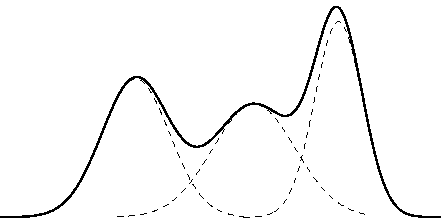
\includegraphics[scale=0.3]{resources/images/gmm}
	\caption{Una combinación de PDFs Gaussianas}
	\label{fig:fig-gmm}
\end{figure}

De lo anterior se desprende que el GMM es parametrizado por los vectores de medias, covarianzas y coeficientes de cada uno de los grupos, siendo expresado como:
$$
\lambda = \{ \omega _i, \mu _i, \Sigma _i \}
$$


Usando un número adecuado de PDF's Gaussianas y ajustando sus parámetros ($\mu _i$ y $\Sigma_i$ ) así como sus coeficientes ($\omega _i$) en una combinación lineal, se obtiene una densidad muy aproximada a la distribución de los datos observados.
% section marco_teórico (end)

\section{Estimación de los parámetros del GMM} % (fold)
\label{sec:estimación_de_los_parámetros_del_gmm}

\subsection{El método de estimación de máxima verosimilitud} % (fold)
\label{sub:el_criterio_de_máxima_verosimilitud}
Existen varios métodos para realizar la estimación de los parámetros $\lambda$ de un GMM, sin embargo el más utilizado es el método de estimación de máxima verosimilitud (ML).

El objetivo del método de ML es maximizar la verosimilitud del GMM dado el conjunto de datos de entrenamiento.

Sea $\mathcal{X}$ una variable aleatoria con función de probabilidad $p(\mathcal{X};\theta)$ donde $\theta$ es un parámetro desconocido.
Además, sean $x_1,x_2,\ldots ,x_N$ los valores observados en una muestra aleatoria de tamaño $N$ de la misma variable.
La función de verosimilitud de la muestra (o función de densidad conjunta) es:
\begin{equation}
\mathcal{L}(\theta) = p(\mathcal{X};\theta) = p(x_1,x_2,\ldots,x_n ; \theta) = \prod_{i=1}^N p(x_i ; \theta)
\end{equation}

La función de verosimilitud es una función de los parámetros de un modelo estadístico que permite realizar inferencias acerca de su valor a partir de un conjunto de observaciones.
El criterio de ML entonces busca elegir el valor adecuado de los parámetros $\theta$ que maximice a $\mathcal{L}$.

Por ejemplo, imaginar que se quiere estimar la probabilidad $p$ de que salga cara en el lanzamiento de una moneda (no necesariamente regular).
Inicialmente, se lanza cinco veces la moneda y se obtiene: $C + C C +$.
Una forma de estimar $p$ sería evaluar la probabilidad de obtener esta muestra para diferentes valores de $p$ y elegir el valor que maximice dicha probabilidad.
Esto puede ser calculado como: $p(C + C C +) = p * (1 - p) * p * p * (1 - p) = p^3 (1 - p)^2$ para todo valor real de P en el intervalo $[0,1]$.
En la Tabla \ref{tbl:ml} se observan los valores obtenidos por distintos valores de $p$.

\begin{table}[h]
\centering
\begin{tabular}{@{}cc@{}}
\toprule
\textbf{Valor de $p$} & \textbf{Probabilidad de la muestra observada} \\ \midrule
0.0                 & 0.0000                                        \\
0.1                 & 0.0008                                        \\
0.2                 & 0.0051                                        \\
0.3                 & 0.0132                                        \\
0.4                 & 0.0230                                        \\
0.5                 & 0.0313                                        \\
0.6                 & 0.0346                                        \\
0.7                 & 0.0309                                        \\
0.8                 & 0.0205                                         \\
0.9                 & 0.0073                                        \\
1.0                 & 0.0000                                        \\ \bottomrule
\end{tabular}
\caption{Valores obtenidos para distintos valores de $p$}
\label{tbl:ml}
\end{table}


El valor que obtiene la máxima probabilidad es 0,6.
Suponiendo que se hayan efectuado $n$ lanzamientos de la moneda obteniendo $k$ caras sin importar el orden en el que han salido, la probabilidad de dicho suceso es dada por:
\begin{equation}
p(k \text{ caras en} n \text{ lanzamientos}) = {n \choose k} p^k (1 - p)^{n-k} = \mathcal{L}(p)
\end{equation}



Si asumimos también que los valores de $n$ y $k$ son conocidos, entonces la verosimilitud queda definida exclusivamente en términos del parámetro $p$.
Como en el caso de cualquier función matemática, la función de verosimilitud puede ser maximizada utilizando las técnicas de cálculo: derivando e igualando a cero y resolviendo las ecuaciones resultantes.

Para el ejemplo los cálculos se simplifican si se representa a $\mathcal{L}$ en términos de logaritmos.
Así a través de la sucesión de ecuaciones \ref{eq:pasos-frec-1}, \ref{eq:pasos-frec-2}, \ref{eq:pasos-frec-3} y \ref{eq:pasos-frec-4} es posible indicar que la frecuencia relativa (ecuación \ref{eq:pasos-frec-4}) es el \emph{estimador máximo verosimil} de la probabilidad de un determinado suceso.
A la serie de pasos efectuados se le conoce como el método de la máxima verosimilitud.
\begin{equation}
\text{ln} \big (\mathcal{L}(p) \big) = k \text{ ln}(p) + (n-k) \text{ ln}(1-p)
\label{eq:pasos-frec-1}
\end{equation}

\begin{equation}
\frac{\partial \text{ ln}\big ( \mathcal{L}(p)  \big )}{\partial p} = \frac{k}{p} - \frac{n-k}{1-p}
\label{eq:pasos-frec-2}
\end{equation}

% \begin{equation}
% \frac{k}{\hat{p}} - \frac{n-k}{1-\hat{p}} = 0 \to k(1-\hat{p}) - \hat{p}(n-k) = 0 \to \hat{p} = \frac{k}{n}
% \label{eq:frec-relativa}
% \end{equation}

\begin{eqnarray}
\frac{k}{\hat{p}} - \frac{n-k}{1-\hat{p}} = 0 &\to& k(1-\hat{p}) - \hat{p}(n-k) = 0 \label{eq:pasos-frec-3}\\ &\to& \hat{p} = \frac{k}{n}
\label{eq:pasos-frec-4}
\end{eqnarray}



Al aplicar este método a muestras que observan una distribución Gaussiana (ecuaciones \ref{eq:pasos-1}, \ref{eq:pasos-2}, \ref{eq:pasos-3}), se observa que los estimadores máximos verosímiles coinciden con la media (ecuación \ref{eq:media}) y la covarianza (ecuación \ref{eq:covarianza}).

\begin{eqnarray}
\mathcal{L}(\mu,\sigma ^2) &=& \text{ln}\prod_{i=1}^N p(x_i;\theta) \label{eq:pasos-1} \\ &=& \text{ ln}\prod_{i=1}^N \frac{1}{\sqrt{2 \pi}\sqrt{\sigma ^2}} \text{exp} \left ( -\frac{(x_i - \mu)^2}{2 \sigma ^2}  \right ) \label{eq:pasos-2} \\ &=&
-\frac{N}{2} \text{ ln}(2\pi \sigma ^2) - \frac{1}{2 \sigma ^2} \sum_{i=1}^{N}(x - \mu)^2 \label{eq:pasos-3}
\end{eqnarray}

\begin{equation}
\hat{\mu} = \frac{1}{N}\sum_{i=1}^{N}x_i
\label{eq:media}
\end{equation}

\begin{equation}
\hat{\sigma}^2 = \frac{1}{N}\sum_{i=1}^{N}(x_i - \hat{\mu})^2
\label{eq:covarianza}
\end{equation}


% subsection el_criterio_de_máxima_verosimilitud (end)


\subsection{El algoritmo EM} % (fold)
\label{sub:el_algoritmo_em}
El algoritmo EM (Expectation-Maximization) se basa en el método de estimación de máxima verosimilitud para determinar los valores \emph{óptimos} de los parámetros ($\lambda$) de un GMM.

Para ello se deben calcular las derivadas de los parámetros de la función de log-verosimilitud $\big(\lambda = \{ \mu_k, \Sigma_k, \omega_k \} \big )$:
$$
\text{ln}p(x|\lambda) = \sum_{i=1}^N\text{ln} \left\{ \sum_{k=1}^{M} \omega _k g \left ( x_i | \mu_k,\Sigma_k \right )  \right\}
$$

Este algoritmo define cuatro pasos básicos:
\begin{enumerate}
	\item Selección de valores iniciales para el parámetro $\big(\lambda = \{ \mu_k, \Sigma_k, \omega_k \} \big )$.
	\item \textbf{Paso Expectation (E)}: Evaluar las probabilidades \emph{a posteriori} utilizando los valores actuales de $\lambda$ .
	\item \textbf{Paso Maximization (M)}: Reestimar los valores de $\lambda$ utilizado las probabilidades \emph{a posteriori} obtenidas.
	\item Evaluar un criterio de parada basado en los valores de las medias o bien en la función de verosimilitud utilizando los nuevos valores del parámetro y compararlos con la iteración anterior.
\end{enumerate}

\subsubsection{Paso 1} % (fold)
\label{ssub:paso_1}
El algoritmo EM requiere la cantidad de $M$ componentes Gaussianas que se desea generar en el GMM.
Esto puede equipararse con la cantidad de grupos que se desea reconocer en el agrupamiento.

Además, requiere el establecimiento de valores iniciales ($\mu_0, \Sigma_0, \omega_0$) en los parámetros. 
Para dicha tarea es posible utilizar un algoritmo de agrupamiento como el \emph{k-means}.
Para el caso de los coeficientes $\omega _k$ sus valores son calculados a través de $\omega _k = N_k / N$ donde $N_k$ es la cantidad de \emph{instancias} del grupo y $N$ es la cantidad total de instancias.

% subsubsection paso_1 (end)

\subsubsection{Paso 2: E} % (fold)
\label{ssub:paso_e}
Para la $i$-ésima muestra se calculan las probabilidades a posteriori para la $k$-ésima componente, o en otras palabras, se calcula la probabilidad de que cada muestra pertenezca a cada clúster, mediante:

\begin{equation}
p(k|x_i,\lambda) = \frac{w_k g(x_i | \mu_k,\Sigma_k)}{\sum_{k=1}^{M} w_k g(x_i|\mu_k,\Sigma_k)}
\end{equation}

donde $g(x|\mu _i,\Sigma_i)  = \frac{1}{(2 \pi)^{(l/2)}}\text{exp} \left(  -\frac{1}{2}(x-\mu _i)^T \Sigma _i^{-1} (x-\mu _i) \right)$.

Este paso puede ser considerado similar al paso de asignación de clúster en el algoritmo k-means.
% subsubsection paso_e (end)


\subsubsection{Paso 3: M} % (fold)
\label{ssub:paso_m}
Se reestiman los valores del parámetro $\lambda$, es decir, $\mu_k, \Sigma_k, \omega_k$, a través de:
\begin{equation}
	\hat{\omega _k}^{t+1} = \frac{1}{N} \sum_{i=1}^{N} p(k|x_i,\lambda)
\end{equation}

\begin{equation}
	\hat{\mu _k}^{t+1} = \frac{\sum_{i=1}^{N} p(k|x_i,\lambda) x_i}{\sum_{i=1}^{N} p(k|x_i,\lambda)}
\end{equation}

\begin{equation}
	\hat{\Sigma _k}^{t+1} = \frac{\sum_{i=1}^{N} p\left(  k|x_i,\lambda \right ) \left( x_i - \hat{\mu}_k^{t+1} \right ) \left( x_i - \hat{\mu}_k^{t+1} \right )^T}{\sum_{i=1}^{N} p\left(  k|x_i,\lambda \right )}
\end{equation}

Este paso puede ser considerado similar al paso de recálculo de clústers en el algoritmo k-means.
% subsubsection paso_m (end)

\subsubsection{Paso 4} % (fold)
Se evalúa la función de log-verosimilitud utilizando los nuevos valores estimados de $\lambda$:

\begin{equation}
	\mathcal{L}(\lambda) = \sum_{i=1}^N \sum_{k=1}^{M} p \left ( k|x_i,\lambda \right ) \left( -\frac{1}{2}(x_i - \hat{\mu}_k)^T \Sigma_k^{-1} (x_i - \hat{\mu}_k) + \text{ ln} P(\hat{w}_k) + c_k \right )
\end{equation}

donde
\begin{equation}
	c_k = - \frac{l}{2}\text{ ln} (2\pi) - \frac{1}{2} \text{ ln}|\Sigma_k|
\end{equation}


Esta evaluación es comparada con la de la iteración anterior y se finaliza la ejecución con los valores actuales si se observa convergencia en la solución.

La convergencia puede ser definida en términos de la diferencia entre las evaluaciones de la función de verosimilitud que debería ser menor a la de un umbral determinado:
\begin{equation}
	|\mathcal{L}(\lambda)_{t-1} - \mathcal{L}(\lambda)_{t}|\leq \epsilon
\end{equation}

Otro mecanismo consiste en observar a los cambios existentes en los valores de $\mu$, deteniendo la ejecución ante la ausencia de cambios o variaciones menores a un umbral.
\label{ssub:paso_4}

% subsubsection paso_4 (end)
% subsection el_algoritmo_em (end)
% section estimación_de_los_parámetros_del_gmm (end)

\section{Conclusiones} % (fold)
\label{sec:conclusiones}
Este documento ha presentado una introducción a las técnicas de agrupación basadas en distribución.
Se ha descrito el funcionamiento del GMM como un exponente de esta categoría de técnicas, así como el algoritmo EM como mecanismo para ajustar los valores de un GMM para así encontrar la pertenencia de cada dato a los clústers participantes en el proceso de agrupación.
% section conclusiones (end)
\newpage 
\nocite{*}
\bibliographystyle{natdin}
\bibliography{references} % expects file "references.bib"

\end{document}